%==============================================================================
%  ENGR 2405 - Electrical Circuits I
%  Lab Report Template
%
%  Compile with pdfLaTeX (or XeLaTeX / LuaLaTeX).
%  If you use the listings code blocks, no extra setup is needed.
%==============================================================================
\documentclass[11pt]{article}

%------------------------- Packages -------------------------------------------
\usepackage[utf8]{inputenc}
\usepackage[T1]{fontenc}
\usepackage[margin=1in]{geometry}     % page margins
\usepackage{amsmath,amssymb}          % math
\usepackage{graphicx}                 % \includegraphics for schematics/scope shots
\usepackage{float}                    % [H] figure placement
\usepackage{booktabs}                 % nicer tables
\usepackage{siunitx}                  % \SI{5}{\ohm}, \SI{10}{\milli\second}, etc.
\usepackage{listings}                 % SciLab / netlist code blocks
\usepackage{xcolor}
\usepackage{caption}
\usepackage[hidelinks]{hyperref}
\usepackage{titlesec}

%------------------------- Section styling ------------------------------------
\titleformat{\section}{\Large\bfseries}{}{0pt}{}
\titlespacing*{\section}{0pt}{1.4em}{0.6em}

%------------------------- Code listing style ---------------------------------
\definecolor{codebg}{RGB}{245,245,245}
\definecolor{codecomment}{RGB}{0,128,0}
\definecolor{codekw}{RGB}{0,0,180}
\lstset{
    backgroundcolor=\color{codebg},
    basicstyle=\ttfamily\small,
    breaklines=true,
    frame=single,
    framesep=4pt,
    keywordstyle=\color{codekw}\bfseries,
    commentstyle=\color{codecomment}\itshape,
    showstringspaces=false,
    captionpos=b,
    tabsize=2,
}
\definecolor{codestr}{RGB}{163,21,21}      % strings
\definecolor{codenum}{RGB}{120,120,120}    % numbers

% --- MATLAB (uses the listings built-in language) -------------------------
\lstdefinestyle{matlab}{
    language=Matlab,
    stringstyle=\color{codestr},
}

% --- SciLab (custom: listings has no built-in SciLab language) -------------
\lstdefinelanguage{Scilab}{
    morekeywords={
        function,endfunction,if,then,else,elseif,end,for,while,do,
        select,case,break,continue,return,clc,clear,disp,mprintf,
        printf,zeros,ones,eye,linspace,inv,det,sum,length,size,abs,
        sqrt,real,imag,exp,sin,cos,tan,plot,plot2d,xlabel,ylabel,
        title,legend,grid,poly,roots,find,pause,error,warning
    },
    sensitive=true,
    morecomment=[l]{//},          % line comment
    morecomment=[s]{/*}{*/},      % block comment
    morestring=[b]",              % double-quoted strings
    morestring=[b]',              % single-quoted strings
}
\lstdefinestyle{scilab}{
    language=Scilab,
    stringstyle=\color{codestr},
}

% --- LTSpice netlist (custom: SPICE directives & comments) -----------------
\lstdefinelanguage{LTspice}{
    morekeywords={
        .tran,.op,.dc,.ac,.step,.param,.model,.lib,.include,.inc,
        .meas,.measure,.save,.backanno,.end,.ends,.subckt,.global,
        .ic,.nodeset,.options,.option,.func,.temp,.four,.noise,.tf
    },
    sensitive=false,
    morecomment=[l]{*},           % lines beginning with * are comments
    morecomment=[l]{;},           % inline ; comments
    morestring=[b]",
}
\lstdefinestyle{netlist}{
    language=LTspice,
    keywordstyle=\color{codekw}\bfseries,
    basicstyle=\ttfamily\small,
}

%==============================================================================
\begin{document}

%------------------------- Title block ----------------------------------------
\begin{center}
    {\LARGE\bfseries LTSpice (Lab 03)\\ENGR 2405}\\[0.8em]
    {\large Abdon Morales}\\[0.3em]
    {\large \today}
\end{center}
\vspace{1em}

%------------------------------------------------------------------------------
\section*{Description}
% Enter a brief description of the lab. This can be taken from the lab
% assignment itself.

This will familiarize the student with the capabilities and basic use of LTSpice which is a freely
available circuit simulation and analysis program, similar to many other Simulation Program
with Integrated Circuit Emphasis (SPICE) programs (e.g. pSpice, ngSpice, etc).

%------------------------------------------------------------------------------
\section*{Calculations}
% Put in any calculations you made. If you used SciLab, paste your program and
% its runtime printout here. Include any reconciliation equations (e.g. mesh
% currents to branch currents) if they are not part of your SciLab output.

The circuit is solved by the matrix form of Ohm's law, $[I] = [R]^{-1}[V]$,
which yields the five mesh currents $i_1$ through $i_5$. The branch currents
measured by LTSpice are then recovered from the mesh currents through the
following relationships:
%
\begin{align}
  I(50\,\Omega) &= i_1 \\
  I(20\,\Omega) &= i_2 - i_1 \\
  I(12\,\text{V}) &= i_3 \\
  I(60\,\Omega) &= i_5 \\
  I(80\,\Omega) &= i_4 - i_1
\end{align}
%
Branches on the outer perimeter of the circuit ($50\,\Omega$, $12$~V,
$60\,\Omega$) belong to a single mesh, so each branch current equals that mesh
current directly. The $20\,\Omega$ and $80\,\Omega$ resistors are shared between
two adjacent meshes, so the current through each is the difference of the two
mesh currents flowing through it. The SciLab program below implements these
equations; its runtime printout follows.

% --- SciLab program ---
\begin{lstlisting}[style=scilab, caption={SciLab program}]
// Calculations for computing the mesh and branch currents
// ENGR 2405 (ECE 402): Electrical Circuits I
// Abdon Morales

R = [150 -20 0 -80 0;
     -20 65 -30 -15 0;
      0 -30 50 0 -20;
     -80 -15 0 95 0;
      0 0 -20 0 80];
disp("R=");
disp(R);

V = [30;
      0;
    -12;
     20;
    -20];
disp("V=");
disp(V);

invR = inv(R);
disp("Inverse of R=");
disp(invR);

disp("This is the vector of mesh currents:");
I = invR * V;
disp(I);

disp("This is the vector of branch currents:");
branchCurrents = [I(1);
                  I(2)-I(1);
                  I(3);
                  I(5);
                  I(4)-I(1)];
disp(branchCurrents);
\end{lstlisting}

% --- SciLab runtime printout ---
\begin{lstlisting}[caption={SciLab runtime output}]
--> exec('/Users/abdonm/Library/CloudStorage/OneDrive-TheUniversityofTexasatAustin/Summer 2026/ECE 402/Lab Notes/Lab 03/lab03.sce', -1)
  "R="
   150.  -20.   0.   -80.   0. 
  -20.    65.  -30.  -15.   0. 
   0.    -30.   50.   0.   -20.
  -80.   -15.   0.    95.   0. 
   0.     0.   -20.   0.    80.
  "V="
   30.
   0.
  -12.
   20.
  -20.
  "Inverse of R="
   0.0173448   0.0132762   0.0088508   0.0167024   0.0022127
   0.0132762   0.0336188   0.0224126   0.0164882   0.0056031
   0.0088508   0.0224126   0.0371639   0.0109921   0.009291 
   0.0167024   0.0164882   0.0109921   0.0271949   0.002748 
   0.0022127   0.0056031   0.009291    0.002748    0.0148227
  "This is the vector of mesh currents:"
   0.7039258
   0.3470378
  -0.1464192
   0.8581014
  -0.2866048
  "This is the vector of branch currents:"
   0.7039258
  -0.3568879
  -0.1464192
  -0.2866048
   0.1541756

\end{lstlisting}

%------------------------------------------------------------------------------
\section*{Simulations}
% Paste (a screenshot is best) your LTSpice schematic and the netlist. Include
% simulation results (graphic outputs, etc.). Node voltages / branch currents
% may be shown on the schematic if the image stays uncluttered; otherwise paste
% the "Simulation Run Results" table here.

\begin{figure}[H]
  \centering
  \setlength{\fboxsep}{8pt}%
  \setlength{\fboxrule}{0.6pt}%
  \fbox{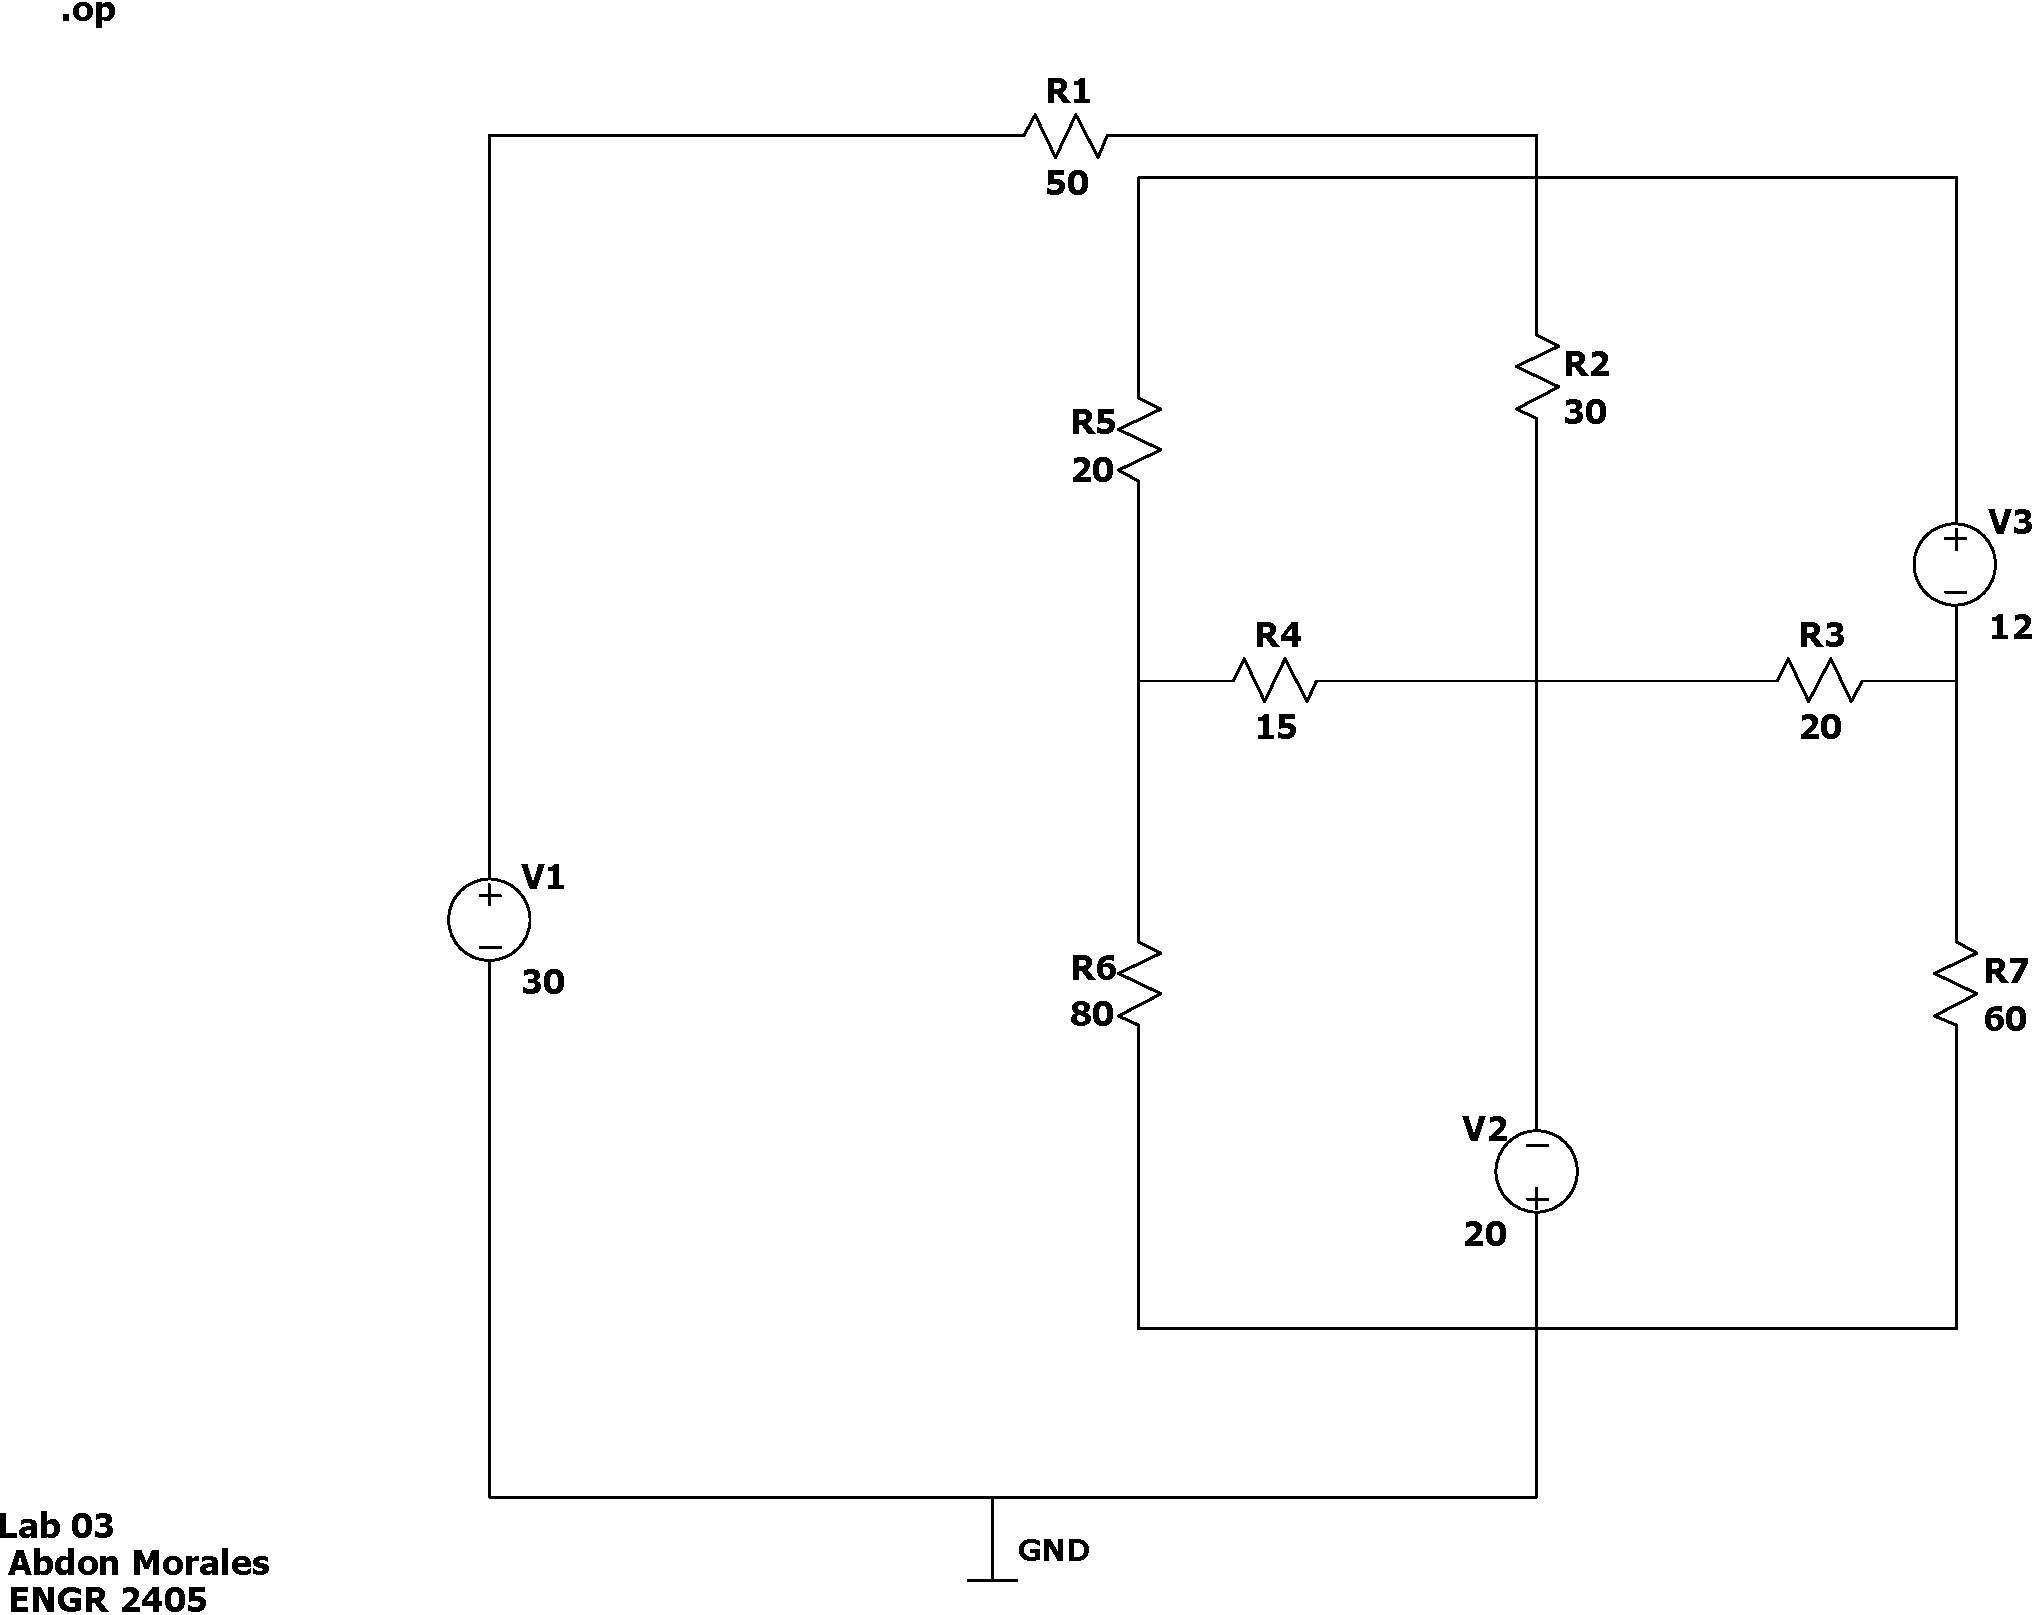
\includegraphics[width=0.8\textwidth]{Lab03-Morales-Abdon-schematic.pdf}}
  \caption{LTSpice schematic}
\end{figure}

\begin{lstlisting}[style=netlist, caption={LTSpice netlist}]
* /Users/abdonm/Library/CloudStorage/OneDrive-TheUniversityofTexasatAustin/Summer 2026/ECE 402/Lab Notes/Lab 03/Lab03-Morales-Abdon.asc
* Generated by LTspice 26.0.2 for MacOS.
V1 N001 0 30
V2 0 N004 20
V3 N002 N005 12
R1 N002 N001 50
R2 N002 N004 30
R3 N005 N004 20
R4 N004 N003 15
R5 N003 N002 20
R6 0 N003 80
R7 N005 0 60
.op
* Lab 03\nAbdon Morales\nENGR 2405
.backanno
.end
\end{lstlisting}

%------------------------------------------------------------------------------
\section*{Results}

The DC operating point simulation produced the following node voltages and device currents:

\begin{verbatim}
--- Operating Point ---

V(n001):    30           voltage
V(n002):    -5.19629     voltage
V(n003):    -12.334      voltage
V(n004):    -20          voltage
V(n005):    -17.1963     voltage
I(R1):      -0.703926    device_current
I(R2):      0.493457     device_current
I(R3):      0.140186     device_current
I(R4):      -0.511064    device_current
I(R5):      -0.356888    device_current
I(R6):      0.154176     device_current
I(R7):      -0.286605    device_current
I(V1):      -0.703926    device_current
I(V2):      -1.14471     device_current
I(V3):      -0.146419    device_current
\end{verbatim}


%------------------------------------------------------------------------------
\section*{Observations \& Discussion}
% List any anomalies or interesting observations. Discuss any discrepancies and
% their reasons. Answer any questions from the lab.

The branch currents computed in SciLab were compared against the LTSpice DC
operating point simulation results, using the mesh-to-branch reconciliation
equations given in the Calculations section. Evaluating those equations from
the SciLab mesh currents and comparing to the LTSpice device currents gives:

\begin{center}
\begin{tabular}{lrrl}
\hline
Branch & SciLab (A) & LTSpice (A) & Agreement \\
\hline
$I(50\,\Omega)$ & $+0.7039$ & $-0.7039$ & magnitude only (sign flipped) \\
$I(20\,\Omega)$ & $-0.3569$ & $-0.3569$ & exact \\
$I(12\,\text{V})$ & $-0.1464$ & $-0.1464$ & exact \\
$I(60\,\Omega)$ & $-0.2866$ & $-0.2866$ & exact \\
$I(80\,\Omega)$ & $+0.1542$ & $+0.1542$ & exact \\
\hline
\end{tabular}
\end{center}

Four of the five branch currents agree exactly, including sign. The only
difference appears in the $50\,\Omega$ resistor (R1), where the magnitude is
identical ($0.7039$~A) but the sign is reversed.

This discrepancy is a sign-convention difference, not a numerical error.
LTSpice reports the current through a two-terminal device as flowing
\emph{into the first node listed for that device in the netlist}. The netlist
entry \texttt{R1 N002 N001} therefore defines positive current as flowing from
N002 to N001 inside R1. The matrix computation instead defines $I(50\,\Omega)=i_1$
using the mesh-current reference direction, which is opposite to the netlist
node ordering for this branch. The two results describe the same physical
current with opposite reference directions, so they differ only in sign. The
remaining four branches happen to have netlist node orderings that agree with
their mesh reference directions, which is why their signs match directly.

The node voltages are also internally consistent: $V(\text{n001}) = 30$~V
corresponds to the positive terminal of the $30$~V source on the far-left node,
with the bottom node taken as ground ($0$~V). The simulation therefore confirms
both the topology and the element values of the circuit.

%==============================================================================
\end{document}
